\documentclass[12pt,a4paper]{article}
\usepackage[utf8]{inputenc}
\usepackage[english]{babel}
\usepackage{amsmath}
\usepackage{amsfonts}
\usepackage{amssymb}
\usepackage{graphicx}
\usepackage{lmodern}
\usepackage{booktabs}
\usepackage{standalone}
\usepackage{tikz}
\usepackage[left=2cm,right=2cm,top=2cm,bottom=2cm]{geometry}
\author{Sergej Kaiser}
\title{Empirical Findings}
\date{\today}
\begin{document}
\maketitle
First the results of estimating $\theta$ with the indicator FD-DVA. Second the tables with the spearman, kendal tau correlation coefficients. 
\begin{table}[htbp] 
\footnotesize
\centering\caption{Cross-Section Results -- Dependent variable FD-DVA}
{
\def\sym#1{\ifmmode^{#1}\else\(^{#1}\)\fi}
\begin{tabular}{l*{5}{c}}
\toprule
            &\multicolumn{1}{c}{(1)}&\multicolumn{1}{c}{(2)}&\multicolumn{1}{c}{(3)}&\multicolumn{1}{c}{(4)}&\multicolumn{1}{c}{(5)}\\
            &\multicolumn{1}{c}{OLS}&\multicolumn{1}{c}{Full Sample}&\multicolumn{1}{c}{Manufacturing Service}&\multicolumn{1}{c}{Without mining}&\multicolumn{1}{c}{EU}\\
\midrule
Log productivity&       -0.09         &       12.87\sym{***}&       16.10\sym{***}&       11.02\sym{***}&       12.73\sym{***}\\
            &      (0.05)         &      (1.15)         &      (2.05)         &      (1.10)         &      (1.39)            \\
Exporter-Importer Fixed Effects & \multicolumn{1}{c}{YES}&\multicolumn{1}{c}{YES}&\multicolumn{1}{c}{YES}&\multicolumn{1}{c}{YES} &\multicolumn{1}{c}{YES}\\
 Importer-Industry Fixed Effects& \multicolumn{1}{c}{YES}&\multicolumn{1}{c}{YES}&\multicolumn{1}{c}{YES}&\multicolumn{1}{c}{YES} &\multicolumn{1}{c}{YES}\\
\midrule
\(N\)       &       15953         &       13663         &       12459         &       13075         &        8918         \\
\(R^{2}\)   &       0.891         &       0.164         &      -0.072         &       0.366         &       0.205         \\
F           &        3.15         &      124.97         &       61.85         &       99.50         &       83.89         \\
widstat     &                     &      143.61         &       78.03         &      122.01         &       96.01         \\
\bottomrule
\multicolumn{6}{l}{\footnotesize Standard errors in parentheses}\\
\multicolumn{6}{l}{\footnotesize \sym{*} \(p<0.05\), \sym{**} \(p<0.01\), \sym{***} \(p<0.001\)}\\
\end{tabular}
}
\end{table}
%\begin{table}[ht]
%\centering \caption{For $\theta_{exgr}=15.29 \quad \text{and} \quad \theta_{FDDVA}=11.02$}
%\begin{tabular}{lccl}
%  \toprule
% & kendal tau & spearman & COU \\ 
%  \midrule
%1 & 0.76 & 0.92 & ARG \\ 
%  2 & 0.54 & 0.73 & AUS \\ 
%  3 & 0.84 & 0.95 & AUT \\ 
%  4 & 0.63 & 0.80 & BEL \\ 
%  5 & 0.75 & 0.90 & BGR \\ 
%  6 & 0.60 & 0.81 & BRA \\ 
%  7 & 0.74 & 0.91 & CAN \\ 
%  8 & 0.69 & 0.85 & CHE \\ 
%  9 & 0.73 & 0.89 & CHL \\ 
%  10 & 0.62 & 0.72 & CHN \\ 
%  11 & 0.61 & 0.82 & COL \\ 
%  12 & 0.74 & 0.88 & CYP \\ 
%  13 & 0.82 & 0.95 & CZE \\ 
%  14 & 0.74 & 0.91 & DEU \\ 
%  15 & 0.73 & 0.89 & DNK \\ 
%  16 & 0.80 & 0.93 & ESP \\ 
%  17 & 0.74 & 0.89 & EST \\ 
%  18 & 0.76 & 0.90 & FIN \\ 
%  19 & 0.66 & 0.86 & FRA \\ 
%  20 & 0.64 & 0.84 & GBR \\ 
%  21 & 0.63 & 0.82 & GRC \\ 
%  22 & 0.60 & 0.75 & HKG \\ 
%  23 & 0.67 & 0.84 & HRV \\ 
%  24 & 0.74 & 0.90 & HUN \\ 
%  25 & 0.54 & 0.76 & IDN \\ 
%  26 & 0.63 & 0.77 & IND \\ 
%  27 & 0.77 & 0.92 & IRL \\ 
%  28 & 0.71 & 0.88 & ISR \\ 
%  29 & 0.81 & 0.95 & ITA \\ 
%  30 & 0.72 & 0.89 & JPN \\ 
%  31 & 0.54 & 0.75 & KOR \\ 
%  32 & 0.85 & 0.96 & LUX \\ 
%  33 & 0.52 & 0.65 & MEX \\ 
%  34 & 0.69 & 0.88 & NLD \\ 
%  35 & 0.61 & 0.78 & NOR \\ 
%  36 & 0.62 & 0.81 & NZL \\ 
%  37 & 0.76 & 0.91 & POL \\ 
%  38 & 0.61 & 0.80 & PRT \\ 
%  39 & 0.79 & 0.94 & SVK \\ 
%  40 & 0.80 & 0.93 & SVN \\ 
%  41 & 0.76 & 0.91 & SWE \\ 
%  42 & 0.68 & 0.81 & TUR \\ 
%   \bottomrule
%\end{tabular}
%\end{table}
%
%\begin{table}[ht]
%\centering\caption{Assuming $\theta_{EXGR}=\theta_{FDDVA}$ }
%\begin{tabular}{lccl}
%  \toprule
% & kendal tau & spearman & COU \\ 
%  \midrule
%1 & 0.76 & 0.92 & ARG \\ 
%  2 & 0.54 & 0.73 & AUS \\ 
%  3 & 0.84 & 0.95 & AUT \\ 
%  4 & 0.63 & 0.80 & BEL \\ 
%  5 & 0.75 & 0.90 & BGR \\ 
%  6 & 0.60 & 0.81 & BRA \\ 
%  7 & 0.74 & 0.91 & CAN \\ 
%  8 & 0.69 & 0.85 & CHE \\ 
%  9 & 0.73 & 0.89 & CHL \\ 
%  10 & 0.62 & 0.72 & CHN \\ 
%  11 & 0.61 & 0.82 & COL \\ 
%  12 & 0.74 & 0.88 & CYP \\ 
%  13 & 0.82 & 0.95 & CZE \\ 
%  14 & 0.74 & 0.91 & DEU \\ 
%  15 & 0.73 & 0.89 & DNK \\ 
%  16 & 0.80 & 0.93 & ESP \\ 
%  17 & 0.74 & 0.89 & EST \\ 
%  18 & 0.76 & 0.90 & FIN \\ 
%  19 & 0.66 & 0.86 & FRA \\ 
%  20 & 0.64 & 0.84 & GBR \\ 
%  21 & 0.63 & 0.82 & GRC \\ 
%  22 & 0.60 & 0.75 & HKG \\ 
%  23 & 0.67 & 0.84 & HRV \\ 
%  24 & 0.74 & 0.90 & HUN \\ 
%  25 & 0.54 & 0.76 & IDN \\ 
%  26 & 0.63 & 0.77 & IND \\ 
%  27 & 0.77 & 0.92 & IRL \\ 
%  28 & 0.71 & 0.88 & ISR \\ 
%  29 & 0.81 & 0.95 & ITA \\ 
%  30 & 0.72 & 0.89 & JPN \\ 
%  31 & 0.54 & 0.75 & KOR \\ 
%  32 & 0.85 & 0.96 & LUX \\ 
%  33 & 0.52 & 0.65 & MEX \\ 
%  34 & 0.69 & 0.88 & NLD \\ 
%  35 & 0.61 & 0.78 & NOR \\ 
%  36 & 0.62 & 0.81 & NZL \\ 
%  37 & 0.76 & 0.91 & POL \\ 
%  38 & 0.61 & 0.80 & PRT \\ 
%  39 & 0.79 & 0.94 & SVK \\ 
%  40 & 0.80 & 0.93 & SVN \\ 
%  41 & 0.76 & 0.91 & SWE \\ 
%  42 & 0.68 & 0.81 & TUR \\ 
%   \bottomrule
%\end{tabular}
%\end{table}
%\begin{table}[ht]
%\centering \caption{For $\theta_{exgr}=15.48 \quad \text{and} \quad \theta_{FDDVA}=11.02$}
%\begin{tabular}{lccl}
%  \hline
% & pearson.fddva.diff.va & spearman.fddva.diff.va & COU \\ 
%  \hline
%1 & 0.75 & 0.91 & ARG \\ 
%  2 & 0.55 & 0.74 & AUS \\ 
%  3 & 0.84 & 0.96 & AUT \\ 
%  4 & 0.66 & 0.82 & BEL \\ 
%  5 & 0.71 & 0.89 & BGR \\ 
%  6 & 0.59 & 0.79 & BRA \\ 
%  7 & 0.73 & 0.91 & CAN \\ 
%  8 & 0.73 & 0.87 & CHE \\ 
%  9 & 0.72 & 0.89 & CHL \\ 
%  10 & 0.63 & 0.73 & CHN \\ 
%  11 & 0.63 & 0.83 & COL \\ 
%  12 & 0.74 & 0.89 & CYP \\ 
%  13 & 0.85 & 0.95 & CZE \\ 
%  14 & 0.73 & 0.90 & DEU \\ 
%  15 & 0.75 & 0.91 & DNK \\ 
%  16 & 0.82 & 0.94 & ESP \\ 
%  17 & 0.73 & 0.88 & EST \\ 
%  18 & 0.77 & 0.91 & FIN \\ 
%  19 & 0.72 & 0.89 & FRA \\ 
%  20 & 0.65 & 0.84 & GBR \\ 
%  21 & 0.63 & 0.83 & GRC \\ 
%  22 & 0.64 & 0.79 & HKG \\ 
%  23 & 0.66 & 0.84 & HRV \\ 
%  24 & 0.73 & 0.91 & HUN \\ 
%  25 & 0.51 & 0.72 & IDN \\ 
%  26 & 0.65 & 0.78 & IND \\ 
%  27 & 0.77 & 0.92 & IRL \\ 
%  28 & 0.69 & 0.86 & ISR \\ 
%  29 & 0.82 & 0.95 & ITA \\ 
%  30 & 0.69 & 0.88 & JPN \\ 
%  31 & 0.51 & 0.72 & KOR \\ 
%  32 & 0.86 & 0.97 & LUX \\ 
%  33 & 0.57 & 0.68 & MEX \\ 
%  34 & 0.71 & 0.88 & NLD \\ 
%  35 & 0.61 & 0.77 & NOR \\ 
%  36 & 0.63 & 0.82 & NZL \\ 
%  37 & 0.78 & 0.91 & POL \\ 
%  38 & 0.68 & 0.86 & PRT \\ 
%  39 & 0.78 & 0.93 & SVK \\ 
%  40 & 0.82 & 0.95 & SVN \\ 
%  41 & 0.78 & 0.92 & SWE \\ 
%  42 & 0.69 & 0.82 & TUR \\ 
%   \hline
%\end{tabular}
%\end{table}

\begin{figure}[hbtp]
\centering
 \includestandalone[width=\textwidth]{graph-ind15-22}
\end{figure}
\begin{figure}[hbtp]
\centering
 \includestandalone[width=\textwidth]{graph-ind23-26}
\end{figure}
\begin{figure}[hbtp]
\centering
 \includestandalone[width=\textwidth]{graph-ind27-35}
\end{figure}
\begin{figure}[hbtp]
\centering
 \includestandalone[width=\textwidth]{graph-ind36-55}
\end{figure}
\begin{figure}[hbtp]
\centering
 \includestandalone[width=\textwidth]{graph-ind57-95}
\end{figure}
\begin{figure}
% Created by tikzDevice version 0.9 on 2015-12-18 02:48:20
% !TEX encoding = UTF-8 Unicode
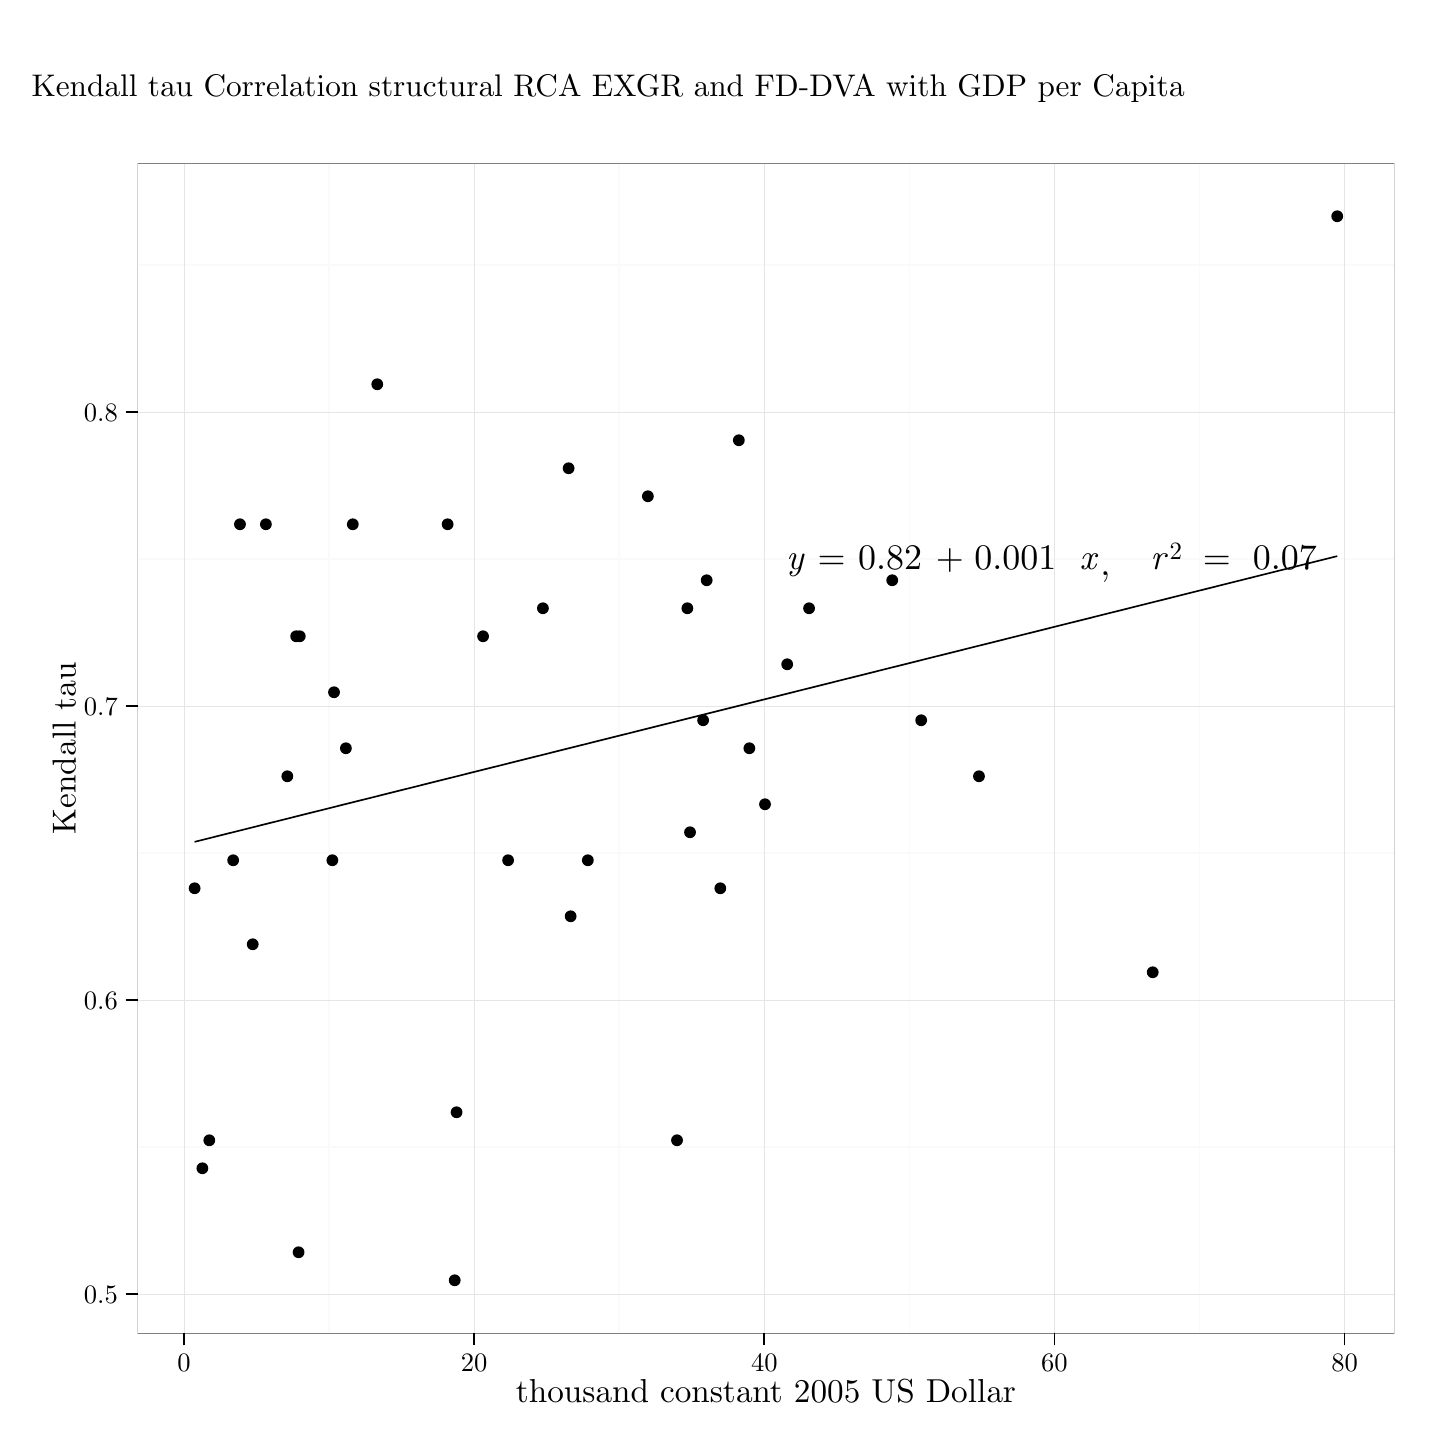
\begin{tikzpicture}[x=1pt,y=1pt]
\definecolor{fillColor}{RGB}{255,255,255}
\path[use as bounding box,fill=fillColor,fill opacity=0.00] (0,0) rectangle (505.89,505.89);
\begin{scope}
\path[clip] (  0.00,  0.00) rectangle (505.89,505.89);
\definecolor{drawColor}{RGB}{255,255,255}
\definecolor{fillColor}{RGB}{255,255,255}

\path[draw=drawColor,line width= 0.6pt,line join=round,line cap=round,fill=fillColor] (  0.00,  0.00) rectangle (505.89,505.89);
\end{scope}
\begin{scope}
\path[clip] ( 39.69, 34.03) rectangle (493.85,456.97);
\definecolor{fillColor}{RGB}{255,255,255}

\path[fill=fillColor] ( 39.69, 34.03) rectangle (493.85,456.97);
\definecolor{drawColor}{gray}{0.98}

\path[draw=drawColor,line width= 0.6pt,line join=round] ( 39.69,101.32) --
	(493.85,101.32);

\path[draw=drawColor,line width= 0.6pt,line join=round] ( 39.69,207.56) --
	(493.85,207.56);

\path[draw=drawColor,line width= 0.6pt,line join=round] ( 39.69,313.80) --
	(493.85,313.80);

\path[draw=drawColor,line width= 0.6pt,line join=round] ( 39.69,420.03) --
	(493.85,420.03);

\path[draw=drawColor,line width= 0.6pt,line join=round] (108.93, 34.03) --
	(108.93,456.97);

\path[draw=drawColor,line width= 0.6pt,line join=round] (213.76, 34.03) --
	(213.76,456.97);

\path[draw=drawColor,line width= 0.6pt,line join=round] (318.60, 34.03) --
	(318.60,456.97);

\path[draw=drawColor,line width= 0.6pt,line join=round] (423.43, 34.03) --
	(423.43,456.97);
\definecolor{drawColor}{gray}{0.90}

\path[draw=drawColor,line width= 0.2pt,line join=round] ( 39.69, 48.20) --
	(493.85, 48.20);

\path[draw=drawColor,line width= 0.2pt,line join=round] ( 39.69,154.44) --
	(493.85,154.44);

\path[draw=drawColor,line width= 0.2pt,line join=round] ( 39.69,260.68) --
	(493.85,260.68);

\path[draw=drawColor,line width= 0.2pt,line join=round] ( 39.69,366.92) --
	(493.85,366.92);

\path[draw=drawColor,line width= 0.2pt,line join=round] ( 56.51, 34.03) --
	( 56.51,456.97);

\path[draw=drawColor,line width= 0.2pt,line join=round] (161.34, 34.03) --
	(161.34,456.97);

\path[draw=drawColor,line width= 0.2pt,line join=round] (266.18, 34.03) --
	(266.18,456.97);

\path[draw=drawColor,line width= 0.2pt,line join=round] (371.02, 34.03) --
	(371.02,456.97);

\path[draw=drawColor,line width= 0.2pt,line join=round] (475.85, 34.03) --
	(475.85,456.97);
\definecolor{fillColor}{RGB}{0,0,0}

\path[fill=fillColor] ( 86.08,326.44) circle (  2.13);

\path[fill=fillColor] (234.64,103.85) circle (  2.13);

\path[fill=fillColor] (256.97,356.80) circle (  2.13);

\path[fill=fillColor] (250.28,194.91) circle (  2.13);

\path[fill=fillColor] ( 76.71,326.44) circle (  2.13);

\path[fill=fillColor] ( 81.32,174.67) circle (  2.13);

\path[fill=fillColor] (245.36,306.21) circle (  2.13);

\path[fill=fillColor] (343.75,235.38) circle (  2.13);

\path[fill=fillColor] ( 97.02,285.97) circle (  2.13);

\path[fill=fillColor] ( 65.63,103.85) circle (  2.13);

\path[fill=fillColor] ( 74.26,205.03) circle (  2.13);

\path[fill=fillColor] (186.18,296.09) circle (  2.13);

\path[fill=fillColor] (126.32,377.03) circle (  2.13);

\path[fill=fillColor] (238.38,296.09) circle (  2.13);

\path[fill=fillColor] (312.40,306.21) circle (  2.13);

\path[fill=fillColor] (195.47,346.68) circle (  2.13);

\path[fill=fillColor] (110.70,265.74) circle (  2.13);

\path[fill=fillColor] (260.78,245.50) circle (  2.13);

\path[fill=fillColor] (239.34,215.15) circle (  2.13);

\path[fill=fillColor] (266.43,225.26) circle (  2.13);

\path[fill=fillColor] (173.60,205.03) circle (  2.13);

\path[fill=fillColor] (196.20,184.79) circle (  2.13);

\path[fill=fillColor] (110.10,205.03) circle (  2.13);

\path[fill=fillColor] (114.99,245.50) circle (  2.13);

\path[fill=fillColor] ( 63.13, 93.73) circle (  2.13);

\path[fill=fillColor] ( 60.33,194.91) circle (  2.13);

\path[fill=fillColor] (322.87,255.62) circle (  2.13);

\path[fill=fillColor] (164.55,285.97) circle (  2.13);

\path[fill=fillColor] (224.11,336.56) circle (  2.13);

\path[fill=fillColor] (244.07,255.62) circle (  2.13);

\path[fill=fillColor] (154.31, 53.26) circle (  2.13);

\path[fill=fillColor] (473.20,437.74) circle (  2.13);

\path[fill=fillColor] ( 97.89, 63.38) circle (  2.13);

\path[fill=fillColor] (274.45,275.85) circle (  2.13);

\path[fill=fillColor] (406.53,164.56) circle (  2.13);

\path[fill=fillColor] (202.41,205.03) circle (  2.13);

\path[fill=fillColor] ( 98.32,285.97) circle (  2.13);

\path[fill=fillColor] (154.98,113.97) circle (  2.13);

\path[fill=fillColor] (117.48,326.44) circle (  2.13);

\path[fill=fillColor] (151.75,326.44) circle (  2.13);

\path[fill=fillColor] (282.35,296.09) circle (  2.13);

\path[fill=fillColor] ( 93.82,235.38) circle (  2.13);
\definecolor{drawColor}{RGB}{0,0,0}

\path[draw=drawColor,line width= 0.6pt,line join=round] ( 60.33,211.69) --
	( 65.56,213.00) --
	( 70.78,214.31) --
	( 76.01,215.61) --
	( 81.24,216.92) --
	( 86.46,218.23) --
	( 91.69,219.53) --
	( 96.91,220.84) --
	(102.14,222.15) --
	(107.37,223.45) --
	(112.59,224.76) --
	(117.82,226.07) --
	(123.04,227.37) --
	(128.27,228.68) --
	(133.50,229.99) --
	(138.72,231.29) --
	(143.95,232.60) --
	(149.18,233.91) --
	(154.40,235.21) --
	(159.63,236.52) --
	(164.85,237.83) --
	(170.08,239.13) --
	(175.31,240.44) --
	(180.53,241.75) --
	(185.76,243.05) --
	(190.99,244.36) --
	(196.21,245.67) --
	(201.44,246.97) --
	(206.66,248.28) --
	(211.89,249.59) --
	(217.12,250.89) --
	(222.34,252.20) --
	(227.57,253.51) --
	(232.80,254.81) --
	(238.02,256.12) --
	(243.25,257.43) --
	(248.47,258.73) --
	(253.70,260.04) --
	(258.93,261.35) --
	(264.15,262.65) --
	(269.38,263.96) --
	(274.61,265.27) --
	(279.83,266.58) --
	(285.06,267.88) --
	(290.28,269.19) --
	(295.51,270.50) --
	(300.74,271.80) --
	(305.96,273.11) --
	(311.19,274.42) --
	(316.41,275.72) --
	(321.64,277.03) --
	(326.87,278.34) --
	(332.09,279.64) --
	(337.32,280.95) --
	(342.55,282.26) --
	(347.77,283.56) --
	(353.00,284.87) --
	(358.22,286.18) --
	(363.45,287.48) --
	(368.68,288.79) --
	(373.90,290.10) --
	(379.13,291.40) --
	(384.36,292.71) --
	(389.58,294.02) --
	(394.81,295.32) --
	(400.03,296.63) --
	(405.26,297.94) --
	(410.49,299.24) --
	(415.71,300.55) --
	(420.94,301.86) --
	(426.17,303.16) --
	(431.39,304.47) --
	(436.62,305.78) --
	(441.84,307.08) --
	(447.07,308.39) --
	(452.30,309.70) --
	(457.52,311.00) --
	(462.75,312.31) --
	(467.98,313.62) --
	(473.20,314.92);

\node[text=drawColor,anchor=base west,inner sep=0pt, outer sep=0pt, scale=  1.3] at (274.09,310) {\itshape y};

\node[text=drawColor,anchor=base west,inner sep=0pt, outer sep=0pt, scale=  1.3] at (285.49,310) {=};

\node[text=drawColor,anchor=base west,inner sep=0pt, outer sep=0pt, scale=  1.3] at (300.12,310) {0.82};

\node[text=drawColor,anchor=base west,inner sep=0pt, outer sep=0pt, scale=  1.3] at (328.19,310) {+};

\node[text=drawColor,anchor=base west,inner sep=0pt, outer sep=0pt, scale=  1.3] at (342.09,310) {0.001};

\node[text=drawColor,anchor=base west,inner sep=0pt, outer sep=0pt, scale=  1.3] at (377.25,310) {};

\node[text=drawColor,anchor=base west,inner sep=0pt, outer sep=0pt, scale=  1.3] at (380.13,310) {\itshape x};

\node[text=drawColor,anchor=base west,inner sep=0pt, outer sep=0pt, scale=  1.3] at (387.62,308) {,};

\node[text=drawColor,anchor=base west,inner sep=0pt, outer sep=0pt, scale=  1.3] at (391.56,310) { };

\node[text=drawColor,anchor=base west,inner sep=0pt, outer sep=0pt, scale=  1.3] at (398.64,310) { };

\node[text=drawColor,anchor=base west,inner sep=0pt, outer sep=0pt, scale=  1.3] at (405.72,310) {\itshape r};

\node[text=drawColor,anchor=base west,inner sep=0pt, outer sep=0pt, scale=  0.9] at (412.61,313.8) {2};

\node[text=drawColor,anchor=base west,inner sep=0pt, outer sep=0pt, scale=  1.3] at (417.57,310) { };

\node[text=drawColor,anchor=base west,inner sep=0pt, outer sep=0pt, scale=  1.3] at (424.65,310) {=};

\node[text=drawColor,anchor=base west,inner sep=0pt, outer sep=0pt, scale=  1.3] at (435.67,310) { };

\node[text=drawColor,anchor=base west,inner sep=0pt, outer sep=0pt, scale=  1.3] at (442.76,310) {0.07};
\definecolor{drawColor}{gray}{0.50}

\path[draw=drawColor,line width= 0.6pt,line join=round,line cap=round] ( 39.69, 34.03) rectangle (493.85,456.97);
\end{scope}
\begin{scope}
\path[clip] (  0.00,  0.00) rectangle (505.89,505.89);
\definecolor{drawColor}{RGB}{0,0,0}

\node[text=drawColor,anchor=base east,inner sep=0pt, outer sep=0pt, scale=  0.96] at ( 32.57, 44.89) {0.5};

\node[text=drawColor,anchor=base east,inner sep=0pt, outer sep=0pt, scale=  0.96] at ( 32.57,151.13) {0.6};

\node[text=drawColor,anchor=base east,inner sep=0pt, outer sep=0pt, scale=  0.96] at ( 32.57,257.37) {0.7};

\node[text=drawColor,anchor=base east,inner sep=0pt, outer sep=0pt, scale=  0.96] at ( 32.57,363.61) {0.8};
\end{scope}
\begin{scope}
\path[clip] (  0.00,  0.00) rectangle (505.89,505.89);
\definecolor{drawColor}{RGB}{0,0,0}

\path[draw=drawColor,line width= 0.6pt,line join=round] ( 35.42, 48.20) --
	( 39.69, 48.20);

\path[draw=drawColor,line width= 0.6pt,line join=round] ( 35.42,154.44) --
	( 39.69,154.44);

\path[draw=drawColor,line width= 0.6pt,line join=round] ( 35.42,260.68) --
	( 39.69,260.68);

\path[draw=drawColor,line width= 0.6pt,line join=round] ( 35.42,366.92) --
	( 39.69,366.92);
\end{scope}
\begin{scope}
\path[clip] (  0.00,  0.00) rectangle (505.89,505.89);
\definecolor{drawColor}{RGB}{0,0,0}

\path[draw=drawColor,line width= 0.6pt,line join=round] ( 56.51, 29.77) --
	( 56.51, 34.03);

\path[draw=drawColor,line width= 0.6pt,line join=round] (161.34, 29.77) --
	(161.34, 34.03);

\path[draw=drawColor,line width= 0.6pt,line join=round] (266.18, 29.77) --
	(266.18, 34.03);

\path[draw=drawColor,line width= 0.6pt,line join=round] (371.02, 29.77) --
	(371.02, 34.03);

\path[draw=drawColor,line width= 0.6pt,line join=round] (475.85, 29.77) --
	(475.85, 34.03);
\end{scope}
\begin{scope}
\path[clip] (  0.00,  0.00) rectangle (505.89,505.89);
\definecolor{drawColor}{RGB}{0,0,0}

\node[text=drawColor,anchor=base,inner sep=0pt, outer sep=0pt, scale=  0.96] at ( 56.51, 20.31) {0};

\node[text=drawColor,anchor=base,inner sep=0pt, outer sep=0pt, scale=  0.96] at (161.34, 20.31) {20};

\node[text=drawColor,anchor=base,inner sep=0pt, outer sep=0pt, scale=  0.96] at (266.18, 20.31) {40};

\node[text=drawColor,anchor=base,inner sep=0pt, outer sep=0pt, scale=  0.96] at (371.02, 20.31) {60};

\node[text=drawColor,anchor=base,inner sep=0pt, outer sep=0pt, scale=  0.96] at (475.85, 20.31) {80};
\end{scope}
\begin{scope}
\path[clip] (  0.00,  0.00) rectangle (505.89,505.89);
\definecolor{drawColor}{RGB}{0,0,0}

\node[text=drawColor,anchor=base,inner sep=0pt, outer sep=0pt, scale=  1.20] at (266.77,  9.03) {thousand constant 2005 US Dollar};
\end{scope}
\begin{scope}
\path[clip] (  0.00,  0.00) rectangle (505.89,505.89);
\definecolor{drawColor}{RGB}{0,0,0}

\node[text=drawColor,rotate= 90.00,anchor=base,inner sep=0pt, outer sep=0pt, scale=  1.20] at ( 17.30,245.50) {Kendall tau};
\end{scope}
\begin{scope}
\path[clip] (  0.00,  0.00) rectangle (505.89,505.89);
\definecolor{drawColor}{RGB}{0,0,0}

\node[text=drawColor,anchor=base west,inner sep=0pt, outer sep=0pt, scale=  1.13] at (  1.39,480.92) {Kendall tau Correlation structural RCA EXGR and FD-DVA with GDP per Capita};
\end{scope}
\end{tikzpicture}
\end{figure}
\begin{figure}
\centering
 \includestandalone[width=\textwidth]{spearman-fddva-diff-exgr}
\end{figure}
\end{document}
